%%%%%%%%%%%%%%%%%%%%%%%%%%%%%%%%%%%%%%%%%%%%%%%%%%%%%%%%%%%%%%%%%%%%%%%%%%%%%%%%%%%%%%%%%%
\documentclass[12pt]{article} %a4paper

\usepackage{graphicx} 
%\usepackage{subfig} 
\usepackage{pdflscape} 
\usepackage{booktabs} 
\usepackage[left=2.5cm,right=3cm,top=3cm,bottom=2.5cm]{geometry}
\usepackage{fancyhdr}
\usepackage[utf8]{inputenc}
\usepackage{float}
\usepackage{datetime}
\usepackage{natbib}
\usepackage{setspace}
\usepackage{booktabs}
\usepackage{color}
\usepackage{multirow}
\usepackage{rotating}
\usepackage{amsmath}
\usepackage{hyperref}
\usepackage{xr}
\usepackage{multicol}
\usepackage{xcolor}
\usepackage{soul}
\usepackage{amsfonts}
\usepackage{subfigure}

\def\citeapos#1{\citeauthor{#1}'s (\citeyear{#1})}

\hypersetup{
    colorlinks,
    linkcolor={red!50!black},
    citecolor={red!50!black},
    urlcolor={blue!80!black}
}
\setlength{\parindent}{0.0in}
\setlength{\parskip}{1.5ex plus 0.5ex minus 0.2ex}
\mmddyyyydate
\doublespacing
\setlength{\columnseprule}{1pt}

\newcommand{\specialcell}[2][c]{%
  \begin{tabular}[#1]{@{}c@{}}#2\end{tabular}}

\externaldocument{tables/ideology_regressions.tex}
\externaldocument{tables/ncsl_crosstab.tex}
\externaldocument{tables/time_diff_reg.tex}

%%%%%%%%%%%%%%%%%%%%%%%%%%%%%%%%%%%%%%%%%%%%%%%%%%%%%%%%%%%%%%%%%%%%%%%%%%%%%%%%%%%%%%%%%%


\begin{document} 


\title{Text as Policy: \\ Measuring Policy Similarity through Bill Text Reuse}
\date{\today}
\author{Fridolin Linder, Bruce Desmarais, Matthew Burgess, Eugenia
Giraudy\footnote{This work was supported by National Science Foundation grants
SES-1558661, SES-1619644, CISE-
1320219 and DGE-1144860. Any opinions, findings, and conclusions or
recommendations are those of the
authors and do not necessarily reflect those of the sponsor.}}

\maketitle

\singlespacing
\begin{abstract} 
    \noindent The identification of substantively similar policy proposals in both proposed and adopted legislation is important to scholars of public policy diffusion and legislative politics. Conventional, manual, approaches are prohibitively costly in constructing datasets that accurately represent policymaking across policy domains, geographic units, and/or time. We propose the use of text-sequencing algorithms, applied to legislative text, to identify bills that introduce similar policy proposals. We present three ground truth tests, applied to a corpus of 500,000 bills from US-state legislatures. First, we show that bills introduced by ideologically similar sponsors are more likely to exhibit a high degree of text reuse. Second, we show that bills classified by the National Council of State Legislatures as covering the same policies exhibit a high degree of text re-use. Third, we show that rates of text reuse across state borders correlate strongly with the diffusion networks recently introduced by Desmarais, Harden and Boehmke (2015).

\end{abstract}

\doublespacing
\clearpage


\section{Introduction} 

The diffusion of public policy has been a central focus in political science research since at least \citet{walker1969}. Research on public policy adoption and diffusion has conventionally relied on modestly-sized, hand-coded datasets that record when a set of jurisdictions adopt one or a handful of similar policies \citep{boehmke2012}. In this paper we draw upon a voluminous and comprehensive source of data with which to measure the consideration and adoption of similar policies -- the text of legislation considered in US state legislatures. We take an automated, text-as-data, approach to the analysis of bill text. This vastly increases the volume of data that can be included in policy adoption research. 

Through the development of automated text-analytic methods of measuring policy diffusion we consider several methodological challenges and broader conceptual hurdles. The central methodological puzzles are two-fold. First, we need to extract segments of text in pieces of legislation that communicate similar policy enactments. Second, we need to develop a method for quantitatively scoring the reused text between bills. The main conceptual puzzle with which we engage is the potential ambiguity regarding whether two policies should be considered the same for the purposes of policy diffusion research. Considering precedents in the literature, we argue for conceptualizing policy adoption in terms of a continuum of similarity rather than a dichotomy of equivalence.

We take a multi-pronged approach to evaluating the performance of text reuse in measuring the consideration and adoption of similar laws. First, we investigate the relationship between the ideological distance of the legislators that proposed two bills and the text reuse scores between these bills. Second, we assess the how well policy diffusion networks that have been established by previous research can be predicted using the amount of text reuse between states. And third, we use data on equivalent bills collected by the National Council of State Legislatures to build an evaluation data set containing true policy overlap to assess the accuracy of text reuse in predicting policy overlap. We find that a high degree of text reuse between bills provides a precise signal of the presence of similar policies within the bills. 


\section{Background}

%%%  Purposes of policy measurement %%% 
The measurement task on which we are focused is the identification of comparable policy actions (e.g., adoption, consideration) across jurisdictions---US states in particular. Scholars of public policy, legislative politics, and related areas have used measurements of comparable policy actions in a variety of research tasks. These include the study of policy diffusion \citep{karch2007emerging}, the comparison of policies on a select legislative issue \citep[e.g., ][]{huber2001legislatures,mycoff2009empirical}, and influence/adoption of model legislation introduced by advocacy organizations \citep[e.g., ][]{garrett2015,burgess2016legislative}. In each of these areas of research, scholars make use of measurements of consistent policy actions across jurisdictions. Below we review a variety of methods, and conceptual definitions that researchers have used in measuring consistent policy actions.

%%% Mechanics of policy measurement %%% 
Public policy research on cross-jurisdiction comparable policy actions has conventionally involved the manual identification of related policies across states, countries or local governments in one or a handful of policy areas \citep[e.g., ][]{walker1969,berry1990,simmons2004,gilardi2009,krause2011policy}. This is a manual approach to measurement at the monadic level. In the area of policy diffusion research, recognizing the limitations of monadic levels of measurement, researchers have developed dyadic approaches to studying the diffusion relationships between states \citep{volden2006,boehmke2009}. In the most recent iteration of dyadic approaches, \cite{desmarais2015} apply network inference algorithms to US state adoption sequences in over 100 policy domains to empirically infer the underlying network through which policies diffuse. In another recent innovation in measurement for policy analysis, \cite{garrett2015} analyze the text of US state legislation to identify the influence of model legislation, as introduced by interest groups.
 
 %%% How has policy similarity been defined, conceptually %%% 
We now consider the coding rules used in past research to define sets of equivalent, or at least similar, policies. Perhaps the broadest approach---studying policies adopted within a domain, but moving the status quo in opposite directions---is represented by \citet{glick1992judicial}. Glick studies judicial enactments related to the ``right to die''---the right of patients or their representatives to end the use of life-preserving medical technology. He considers an adoption to include any judicial enactment on this topic, whether they restrict medical providers' deference to the patients or enact broad patients' rights.  \citet{berry1990} look at policy change in a uniform direction---states' adoption of lotteries. Lotteries, of course, vary in terms of their rules and financial models, but all of the policies studied by \citet{berry1990} moved the status quo from no state lottery to the existence of a state lottery. \citet{volden2006} considers a broad array of state laws---those implemented for the Federal Health and Human Services Children's Health Insurance Program (CHIP). CHIP laws were coded for six policy characteristics and then analyzed for diffusion dynamics. Lastly, \citet{mooney1995legislative} provides an example of quantitative coding of policies adopted in a given domain. They code the permissiveness of state abortion laws (pre Roe v. Wade) on a five-point scale. These examples convey the variability with which scholars have defined the set of policies that are considered to be comparable across state borders.


\section{Detecting Policy Similarity through Text Reuse}

The above review of the ways in which researchers have defined comparable policies offers clarity regarding the implicit concepts underlying policy comparability. We see that policies that are considered comparable exhibit two qualities. First, they often, but do not always, move the status quo in a similar direction. This could be thought of as ideological similarity. Second, they enact policy in similar domains---either narrowly or broadly conceived. Before we describe the algorithm we use for detecting text re-use, and validate that algorithm, we draw upon these two concepts to define the latent variable we seek to measure through the assessment of text overlap. Specifically, we are motivated by the fact that researchers do not typically focus on strictly equivalent policies. Rather, they deem policies comparable if they are highly similar along one or two dimensions---policy domain and (optionally) ideological direction. 

We see past work that has identified sets of comparable policies as focusing on sets of policies that meet some threshold of similarity. As such, the latent variable that we argue below is measured effectively through text re-use is {\em policy similarity}. The text in legislation is an aggregate representation of the dimensions underlying the policies proposed therein. These dimensions include the domain of the policy, the ideological position enacted by the policy, the level of specificity in the policy enactment, and several other salient features of policy that are communicated through the text in legislation. We do not claim that the re-use of text can be used to measure these dimensions in a specific, dis-aggregated way. Rather, text re-use serves as a summary measure of the greatest overlap observed across all relevant policy dimensions represented in legislative text. 

\subsection{Detecting Text Reuse}
\label{sec:d_t_r}
To assess the maximal similarity of policies proposed in two pieces of legislation, we seek to identify large segments of equivalent or highly similar text (i.e., text reuse between bills). Alignment algorithms for discovering similar long sequences of text stand in contrast to bag-of-words methods, which are based on the comparison of word occurrence frequencies in documents. Bag-of-words methods may be effective for capturing broad topical areas in legislation, but will provide results that are too coarse for precisely assessing policy overlap. For example, in modeling bills in the US Congress using statistical topic models, arguably the canonical bag-of-words method for text analysis, \citet{gerrish2011predicting} find that topic models for legislative text perform most effectively when parameterized with 64 topics to model a corpus of 4,447 bills. While 64 topics provides a fairly detailed categorization of the domains covered in legislation, it is unrealistic to think that this method can isolate individual policy proposals.  Considering \citeapos{gerrish2011predicting} results again, that would mean that the US Congress considers nearly seventy bills, on average, for each specific policy proposed. 

There are a variety of algorithms designed to automatically detect text reuse between documents mostly originating in the plagiarism detection literature \citep[see e.g.][for an overview]{potthast2013overview}. In political science, \citet{wilkerson2015tracing} introduced the Smith-Waterman local alignment algorithm (SW algorithm) to detect overlapping language in congressional bills in order to trace policy ideas through the legislative process of the US Congress. We use the same algorithm to detect text reuse in US state bills, however, our implementation of the algorithm differs slightly. The SW algorithm was developed by \citet{smith1981identification} in molecular biology, in order to match genetic sequences. Given two sequences (of genes or words) it calculates the optimal alignment (match) between these sequences. 

Sequences in text that convey equivalent content matter often do not match perfectly. Formatting, white space, typographical errors, etc. would decrease the precision dramatically if only exact matches were used. The SW algorithm, therefore, returns the optimal alignment while allowing for mismatches and gaps. The extent to which such imperfections are tolerated is governed by parameters that are set by the researcher. There are three such parameters: the match score (reward for exactly matching words), the mismatch score (penalty for including words that do not match), and the gap score (penalty for including placeholder words in matching a shorter sequence to a longer sequence). The goal of the algorithm is to return the the alignment with the highest score given the input sequences and the parameters. Consider the following two excerpts from Alaska State Bill 203 (28th session) and North Carolina House Bill 366 (2015) respectively:

\begin{quote}
\textit{"section 1.AS44.99 is amended by adding new sections to read: article 6. compact for a balanced budget (...)"} \\
\textit{"chapter 143 is amended by adding a new article to read: article 80. compact for a balanced budget (...)"}
\end{quote}

There is a large number of possibilities of how these sequences could be aligned. There is a trade-off between short sequences that match perfectly, and longer sequences with imperfections. For example, we could match just ``is amended by adding new'' or ``compact for a balanced budget''. However, by adding a gap between ``adding'' and ``new'' in the first sequence and accepting the mismatches ``article''-``section'' and ``6.''-``80.'', a longer alignment can be obtained: ``is amended by adding \textit{(a)} new \textit{(article/section)} to read: article \textit{(6./80.)}''. 

Because there are so many different possibilities, it is computationally demanding to find the optimal alignment. \citet{smith1981identification} therefore proposed a dynamic programming approach that is illustrated in Figure \ref{fig:score_matrix}. Dynamic programming refers to algorithms that divide a problem into sub-problems and store results of previous calculations for later ones. In the case of the SW algorithm, the property that makes it a dynamic problem is the fact that all the alignments of shorter sub-sequences of an optimal alignment of a sequence are themselves optimal. Intuitively, if the benefits of including a sub-sequence in an alignment outweigh the penalties from mismatches and gaps in that sub-sequence, that sub-sequence will contribute positively to longer alignments to which it is appended. To make this clearer consider the beginning of the sequences in the example above:

\begin{quote}
\textit{``section 1.AS44.99 is amended''}\\
\textit{``chapter 143 is amended''}
\end{quote}

It is obvious that the best local alignment of the first three elements would be just "is" - "is" since the first two elements don't match and therefore would just reduce the overall quality of the alignment. If we now consider the alignment of the first four words we know that we can discard all possible alignments that involve the first two elements because the quality of every alignment that involves these elements could be improved by dropping them. Re-using the result from the first three elements, the problem of aligning the first four elements is now reduced to the single decision about the elements ``amended'' and ``amended''. This decision is easy to make because we only have to consider four possibilities: We match the elements and they are actually the same, we match the elements and they are not the same, we introduce a gap in one of the sequences or we decide to stop the alignment. 

If the next two elements match, the decision is easy - we add them and increase the total alignment score. However, if they do not match the decision is more difficult. We only want to introduce a gap or mismatch if it pays off later (that is if we thereby can `reach' another part of the sequence that matches again). But we only know that once we went through the whole sequence. The central idea is therefore to find all optimal alignments ending in all possible spots, keep these scores and after everything is calculated finding the alignment that maximizes the overall quality. Therefore, after the decision is made the same procedure is applied to the next pair of sequence elements, and repeated until the end of both sequences is reached.

This intuition can be formalized in an algorithm that is based on a dynamic programming matrix that contains all optimal sub-alignments. A matrix is created where each combination of elements of the two sequences is assigned a cell. And an additional row and column of 0 is appended to the beginning of each sequence (to allow for a gap in the beginning of one sequence). The quality or alignment score of every possible alignment is then calculated cumulatively with the following algorithm. Denote the two sequences as $\mathcal{A} = (a_1, a_2, ... a_n)$ and $\mathcal{B} = (b_1, b_2, ..., b_k)$. Additionally let $\delta$, $\epsilon$ and $\gamma$ be the match, mismatch and gap scores. Define the scoring function:
\begin{equation}
	\label{eqn:scoring}
	S(a_i, b_j) = \delta^{\mathbb{I}(a_i = b_j)} + \epsilon^{\mathbb{I}(a_i \neq b_j)}
\end{equation} 
Where $\mathbb{I}(.)$ is the indicator function. Then the entry for each cell $M_{i,j}$, $i=1,2,...,n$ and $j=1,2,...,k$ of the matrix is filled by the following rule:
\begin{equation}
	\label{eqn:fill}
	M_{i,j} = \max(M_{i-1,j-1} + S(a_i, b_j), M_{i-1,j} + \gamma, M_{i,j-1} + \gamma, 0)
\end{equation}

The algorithm is visualized for the example above in Figure
\ref{fig:score_matrix}\footnote{An interactive version can be found at
    \url{http://fridolin-linder.com/2016/03/30/local-alignment.html}.}. Each row corresponds to a word in the sentence from the Alaska bill and each column to the sentence from the North Carolina bill. On the right side of the matrix the optimal alignment is displayed.

\begin{figure}[ht!]
	\centering
	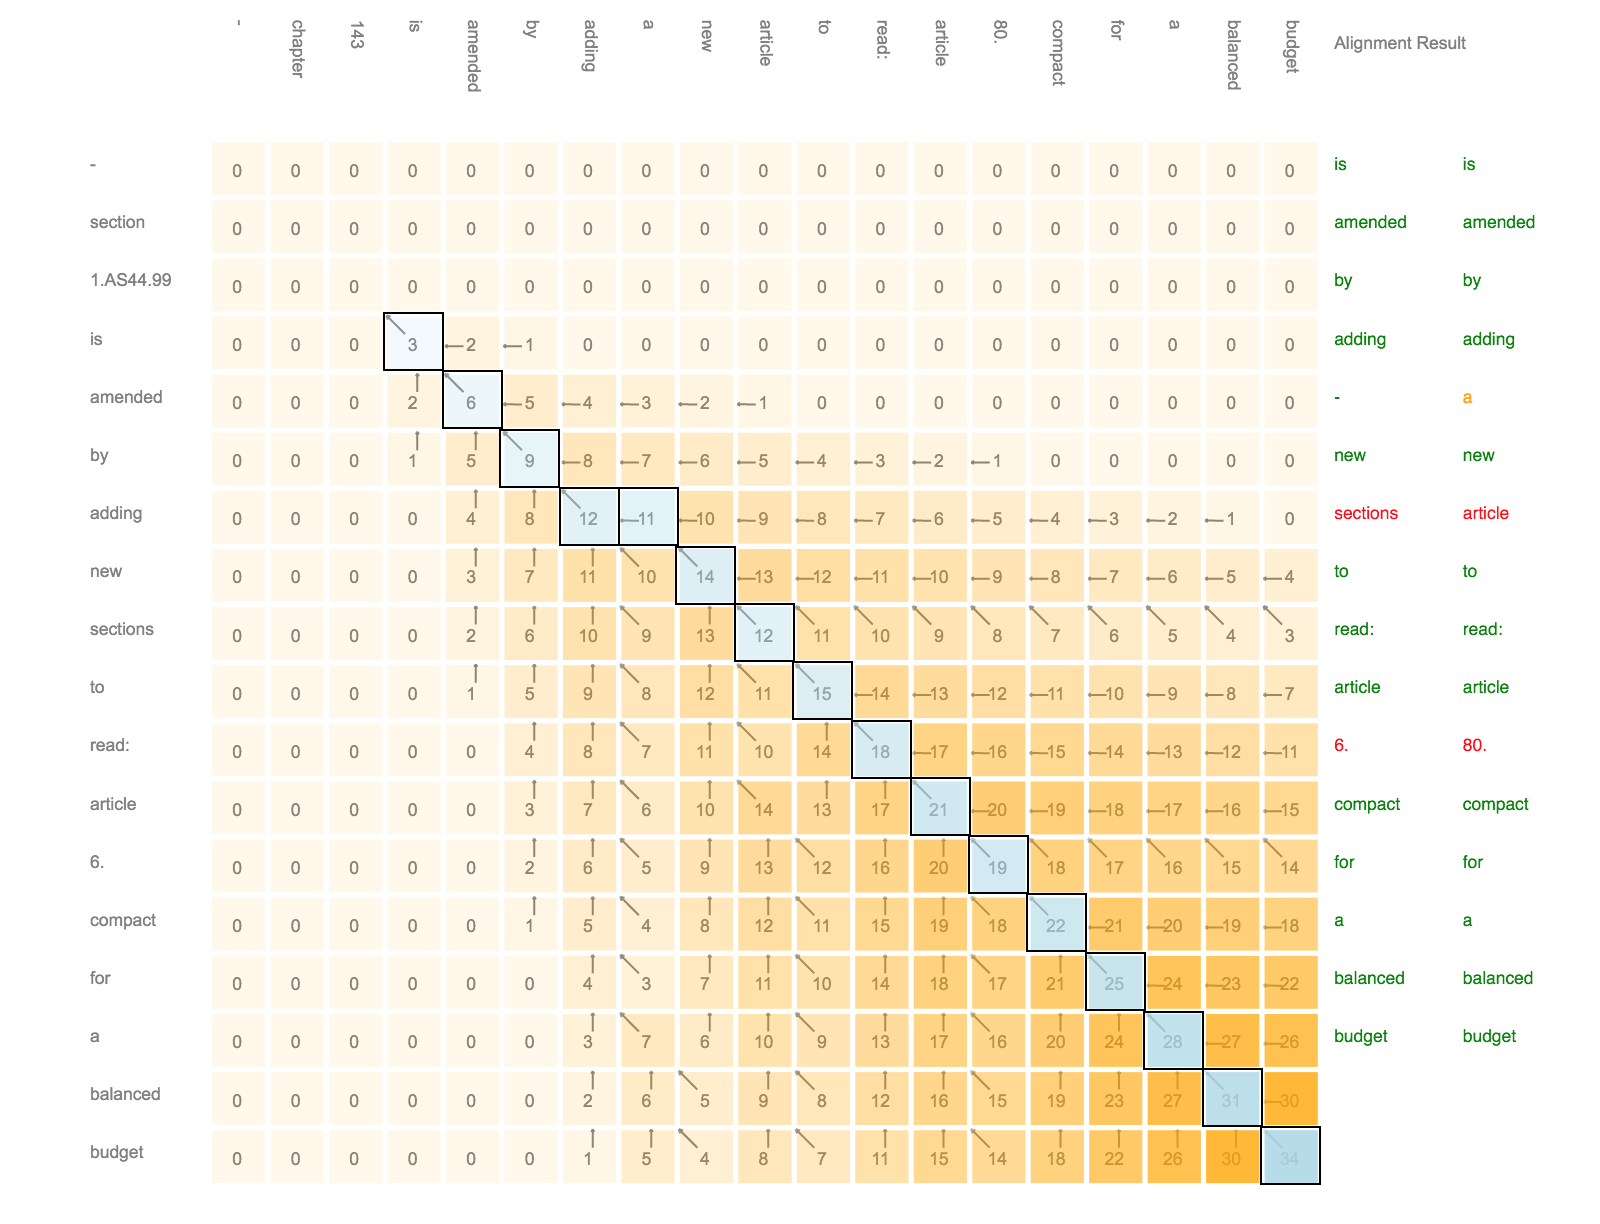
\includegraphics[width=1.05\textwidth]{figures/sm.png}
    \caption{Dynamic programming array of local alignment algorithm. The parameters in this instance are: Match Score: 5, Mismatch Score: -2, Gap Score: -1. The optimal alignment is displayed on the right side of the matrix. The left column corresponds to the text sequence in the rows of the matrix, the right column to the sequence in the columns. Mismatches are colored in red, gaps are indicated by "-" and orange color. The blue cells in the matrix display the path of the optimal alignment.}
    \label{fig:score_matrix}
\end{figure}

The four values of which the maximum is chosen in Equation \ref{eqn:fill}
describe four steps in this dynamic programming array. The first value
corresponds to a diagonal step which means in the resulting alignment sequence
elements $a_i$ and $b_j$ are matched and the score of the alignment is either
increased by $\delta$ if they match or decreased by $\epsilon$ if they don't
match. The second and third value describe a gap step either in horizontal or
vertical direction. That is, if we move from cell $(i,j)$ to cell $(i+1,j)$, in
the resulting alignment sequence element $a_{i+1}$ is matched with a gap. On the
other hand, if we move to cell $(i, j+1)$ sequence element $b_{j+1}$ is matched
with a gap in the resulting alignment. If the first three values are all $<= 0$,
the score in the cell is 0 meaning that no step is taken and every potential
alignment stops at this point. This can be observed in Figure \ref{fig:score_matrix}. The blue path describes the optimal alignment. The first two elements in both sequences don't match, therefore the score remains zero. Therefore the resulting alignment starts at the fourth element of each sequence with four diagonal steps, each adding points $(\delta = 5)$ to the final score which reaches 20 at the alignment ending in ``adding''-``adding''. After that, a step to the right is taken, meaning that the additional ``a'' in the column sequence is matched with a gap in the row sequence (indicated by ``-'' and orange coloring in the result on the right hand side). The cumulative score of the alignment is reduced by $\gamma = -1$ to 19. After that only diagonal steps are taken. Note that there are two mismatches each of which reduces the score by $\epsilon = -2$. 

The optimal alignment is identified by finding the highest score in the matrix,
at which the alignment ends, and back-tracing the path of the alignment. The
steps in the path are chosen using Equation \ref{eqn:fill}, and are indicated in
Figure \ref{fig:score_matrix} by arrows pointing to the left, the upper left, up
or no arrow. The back-tracing continues until a  zero is encountered.

This algorithm is computationally intensive ($\mathcal{O}(nk)$ in computation
time and memory demand), but returns the globally optimal local alignment given the scoring parameters. We provide a proof of this in the appendix. The property follows from the recursive relation used to fill the dynamic programming matrix. An alignment that is constructed by adding one element to an already optimal alignment is optimal itself. Starting by aligning the first two elements of the sequence optimally (which is trivial), a globally optimal can be found by iteratively adding to this alignment.

In our analyses we use a slightly modified version of the local alignment algorithm, in which the first gap in a series of multiple gaps receives a higher penalty then the following ones \citep[][use the same modification]{wilkerson2015tracing}. This penalizes many small gaps and makes the algorithm produce longer gaps. The idea behind this modification is that someone who changes text in a bill might insert several words into an existing piece of text. The fact that something was inserted should weigh heavier than the length of the insertion which is achieved by down-weighting gap extensions. 




\section{Policy Similarity in US State Legislation}
% What we will provide through the application of the SW algorithm?
Through the application of the SW algorithm to US state legislation, we will
provide a quantitative measure of policy similarity between bills. The
similarity measures between bills  that we identify can be aggregated up to the legislator or state levels. The measures we provide can be used to test hypotheses regarding, among other topics, public policy diffusion, legislative politics, political parties, and interest groups.  

\subsection{Data}
We apply the SW algorithm to a database of US state bills, collected by
\citet{burgess2016legislative} and the Sunlight
Foundation\footnote{\url{http://sunlightfoundation.com/}}. This data base
contains approximately 500,000 bills from 2008 to 2015\footnote{Since
    computation is very demanding for this problem, the results reported in this
    version of the paper are based on a random sample of about half of the
    bills. We are in the process of completing the analyses for the whole
dataset.}. Not all bills from all
states are available for the whole time period. Figure \ref{fig:bill_desc}
displays the year ranges and number of bills in the bill data base. This
collection of bills is based on all bills that are available through the
Sunlight Foundation's \url{openstates.org} API. \url{openstates.org} is a website maintained by the Sunlight Foundation, in order to increase transparency in state politics. The Sunlight Foundation uses web scrapers to access all bills that are available on the websites of legislatures in all US states. This includes enacted legislation as well as bills that are still in the legislative process, or where not enacted. %The database contains the bill text as well as additional information on the legislative process for the bill. We have the first and the last version of the bill text, the sponsor of the bill and all legislative action that was taken on the bill. %The available meta-data for the bills includes a time-stamp for introduction and approval of the bill, the name and party affiliation of the sponsor(s), the state and the bill id.

\begin{figure}[ht!]
    \centering
    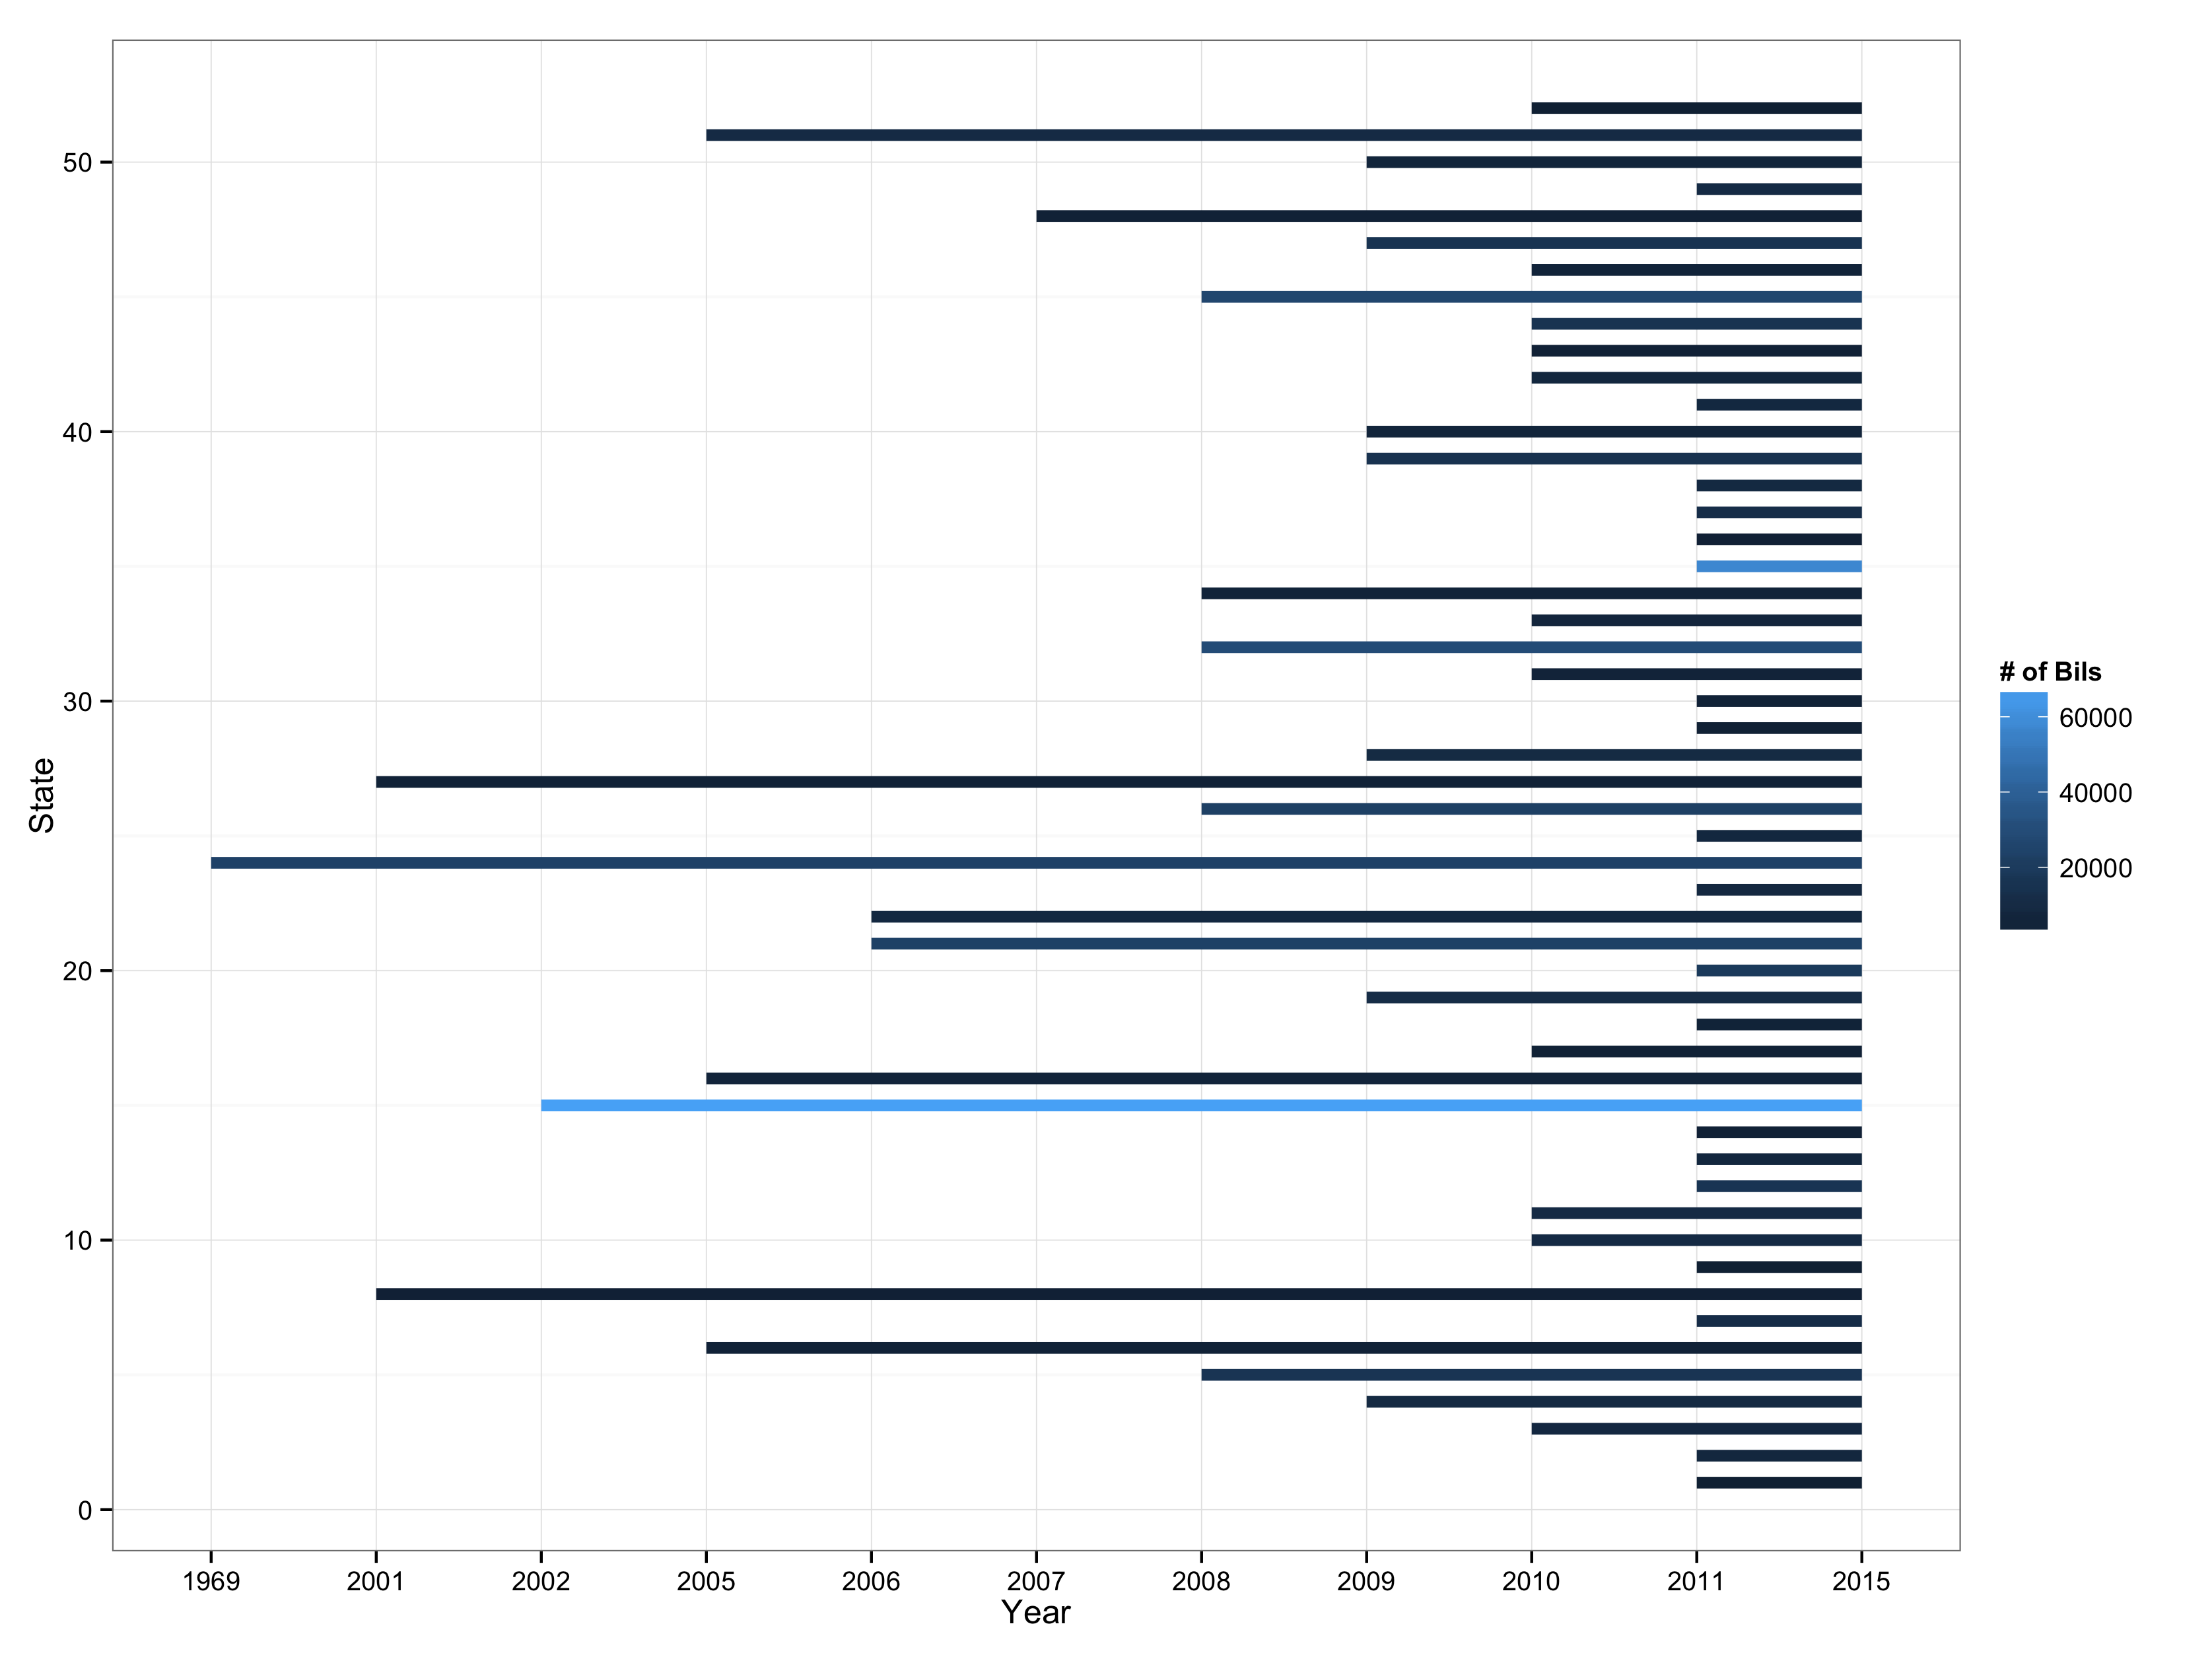
\includegraphics[width=0.65\textwidth]{figures/year_count_by_state.png}
    \caption{Description of the bill database. The horizontal bars display the time range for which bills are available for each state. The color of the bar indicates how many bills are available for this state.}
    \label{fig:bill_desc}
\end{figure}

Our approach of applying the SW algorithm is similar to
\citet{wilkerson2015tracing} but differs in several key respects. The analysis
consists of three major steps: 1) Pre-processing and selection of documents to compare, 2) alignment computation, 3) post hoc refinement (boiler plate removal). 




\subsection{Pre Processing and Selection}

The SW algorithm is computationally demanding and an exhaustive comparison of
all possible bill-pairs is not feasible (with $500,000$ bills this would amount
to about $124 * 10^9$ bill pairs). \citet{wilkerson2015tracing} encountered the same problem and excluded bills that don't have at least five matching 10-grams. Since this implies considerable exact character matches, we see this as a too restrictive for our application. Because the text we are using originates in 50 different legislatures, exact character matches might obfuscate valuable text reuse just because of small formatting changes, changes of state names, etc. 
Instead we choose to rely on a procedure that is based on finding bills with
similar language. We store all available bills in an Elastic Search database.
Elastic search is an open source web search engine which is designed to find
document that match a search query \citep{gormley2015elasticsearch}. We utilize
the `more like this' query, which is designed to find documents that are similar
to a given document. It works in the following way: From the focus document, the
$k$ $n$-grams with the highest tf-idf scores are selected and transformed into a
search vector that is representative of the query document. Then, for each
document in the collection, a variation of the cosine similarity is calculated
and the $m$ bills with the highest scores are selected for further analysis. For
this analysis we set $k$ to 25, $n$ to 5 and $m$ to 1000\footnote{For
details on the exact algorithm we refer the reader to the elastic search
documentation (\url{http://sunlightfoundation.com/} as well as the lucene engine
documentation
(\url{https://lucene.apache.org/core/4_9_0/core/org/apache/lucene/search/similarities/TFIDFSimilarity.html}).
In order to account for the possibility of selection bias being introduced to
our analyses through the cap of 1000 similar bills, we analyzed the results with
different numbers of pre-selected bills. We find that this parameter, when set
to a sufficiently high value, does not lead to such bias because the set of
potentially relevant bills is always much smaller than 1000.}


\subsection{Bill Alignment Computation}

Once the candidate bills are selected, the alignments are calculated for all
possible bill-dyads, bill pairs from the same state are available but excluded
for the analyses below. We exclude same-state comparisons in the current analysis since our validation exercises are focused on cross-state comparisons. We refer to the two sections involved in each alignment process as `left' and `right' sections. The algorithm returns parts of the left and right section that are determined to be aligned as well as a score. We refer to these three pieces of information as an alignment. 

\clearpage

\begin{table}[ht!]
\centering
\caption{Alignment Examples. Yellow highlighting shows matching sections. Dashes stand for gaps introduced by the alignment algorithm. Non highlighted text are mismatches.}
\label{tab:alignment_examples}
\bgroup
\def\arraystretch{2}
\begin{tabular}{p{0.45\textwidth}|p{0.45\textwidth}|p{0.1\textwidth}}
Left Text & Right Text & Score\\
\hline

\textbf{nj\_214\_A1167}: "\hl{the entire credit may not be taken for the taxable year in which the} renewable energy property \hl{is placed in service but must be taken in five equal} - \hl{installments beginning with the taxable year in which the} renewable energy property \hl{is placed in service. if, in one of the years in which the installment of a credit accrues, the} renewable energy property \hl{with respect to which the credit was claimed is disposed of}, \hl{taken out of service, or moved out of state, the credit expires and the taxpayer may not take any remaining installment of the credit. the taxpayer may, however, take the portion of an installment that accrued in a previous year and was carried forward to the extent permitted under}" & \textbf{nc\_2011\_SB747}: "\hl{the entire credit may not be taken for the taxable year in which the} facility - - \hl{is placed in service but must be taken in five equal} annual \hl{installments beginning with the taxable year in which the} facility - - \hl{is placed in service. if, in one of the years in which the installment of a credit accrues,} the facility - - \hl{with respect to which the credit was claimed is disposed} - - - \hl{of} - \hl{or taken out of service, the credit expires and the taxpayer may not take any remaining installment of the credit. the taxpayer may, however, take the portion of an installment that accrued in a previous year and was carried forward to the extent permitted under}" & $388$ \\

\textbf{nj\_214\_A1167}: "\hl{the entire credit may not be taken for the} taxable \hl{year in which the} renewable energy \hl{property is placed in service but must be taken in} five \hl{equal installments} - - - - - \hl{beginning with the taxable year in which the}" & \textbf{ga\_2011\_12\_HB146}: "\hl{the entire credit may not be taken for the} - \hl{year in which the} - - \hl{property is placed in service but must be taken in} four \hl{equal installments} over four successive taxable years \hl{beginning with the taxable year in which the}" & 110 \\

\textbf{nj\_214\_A1167}: "\hl{the entire credit may not be taken for the taxable year in which the}" renewable energy property is placed in service \hl{but must be taken in five equal installments beginning with the taxable year in which the} & \textbf{nc\_2009\_SB305}: "\hl{the entire credit may not be taken for the taxable year in which the} costs are paid - - - - \hl{but must be taken in five equal installments beginning with the taxable year in which the}" & 108\\
\hline
\end{tabular}
\egroup
\end{table}

\clearpage

From this procedure we obtain ca. $1.2 * 10^8$ individual alignments (that is, shared
text between two bills). Figure \ref{fig:alignment_score_distribution} displays the cumulative frequency
distribution of the alignments. The vast majority of alignments are very small
(less than 50). Table \ref{tab:alignment_examples} displays three examples of alignments. The `Left Text' and `Right Text' columns display the optimal alignment for the two sections the alignment score is displayed in the `Score' column. This example shows the reuse of legislative text in three states (New Jersey, North Carolina and Georgia).


\begin{figure}[ht!]
    \centering
    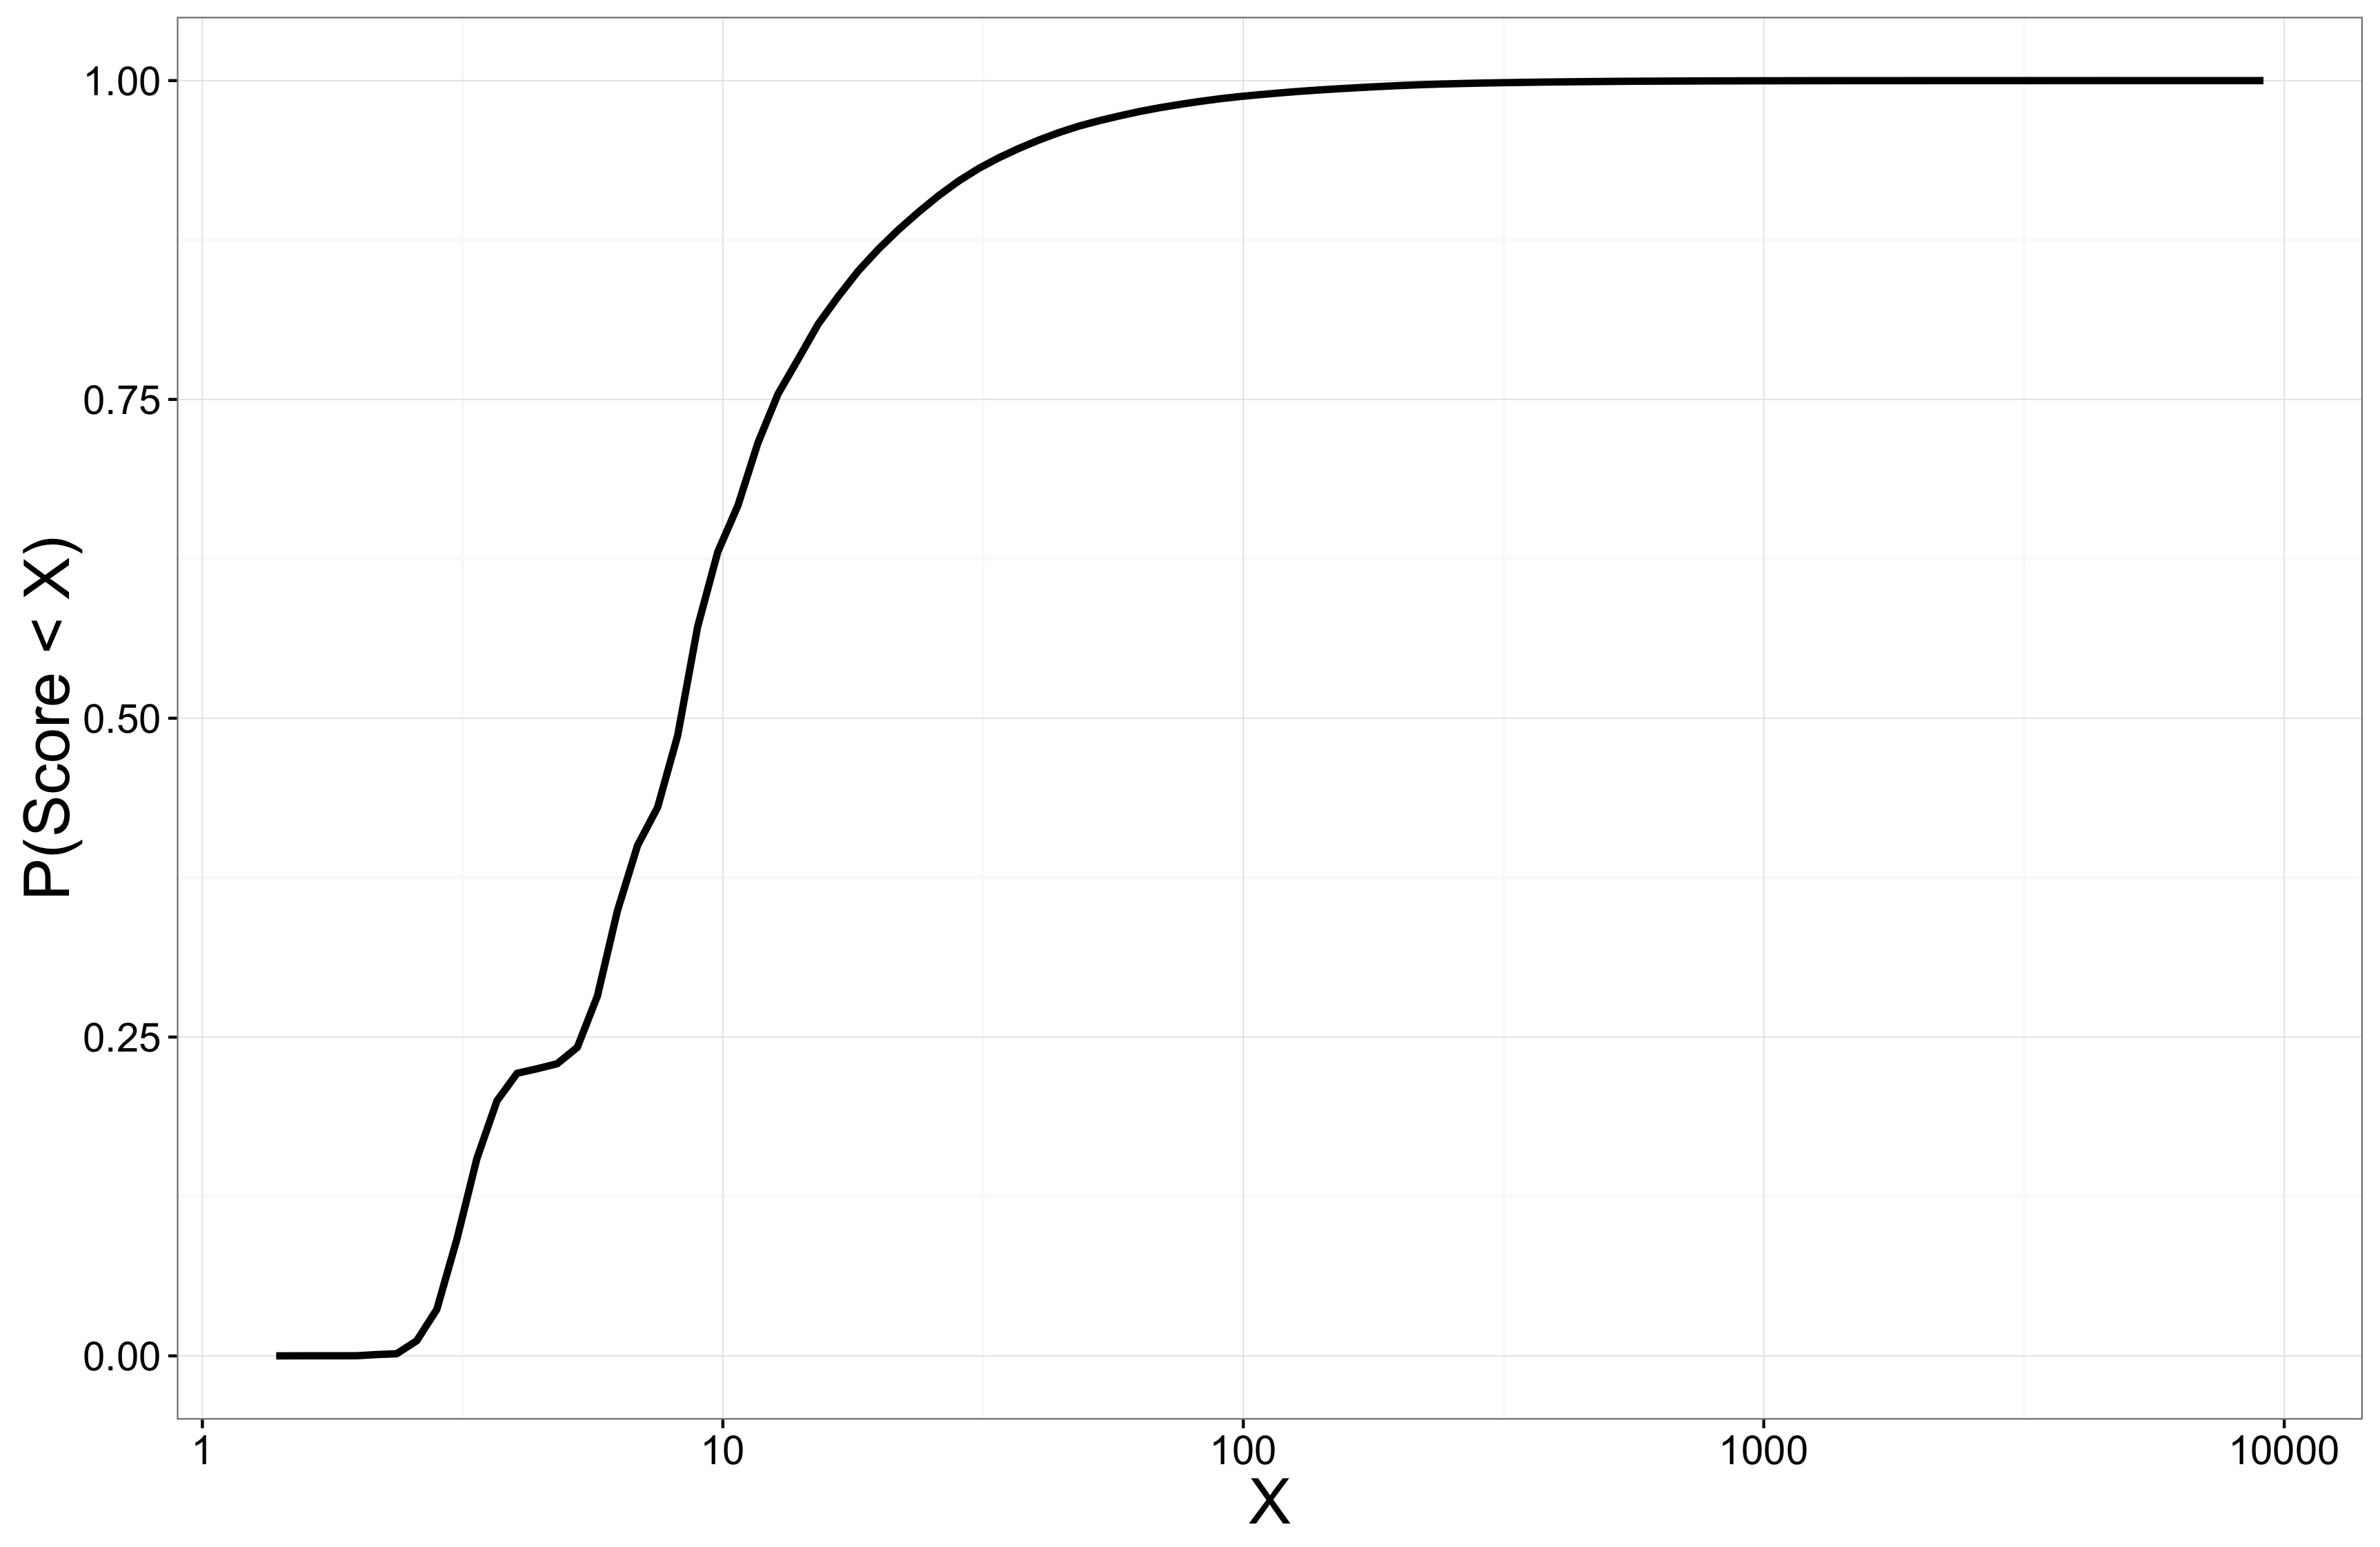
\includegraphics[width=0.8\textwidth]{figures/alignment_score_distribution.png}
    \caption{Cumulative frequency distribution of the dyad level alignment
    scores. The x-axis represents the dyad level alignment score on the
    $log_{10}$ scale.}
    \label{fig:alignment_score_distribution}
\end{figure}



\subsection{Approaches to Adjusting for Boiler Plate Text}

Legislation is full of textual content that is not very useful in identifying the novel policy proposal(s) offered by the bill. Such text includes procedural language, headers, section titles, and common phrases such as definitions of legal terms, tax brackets, etc. Text that is irrelevant to specific policy proposals represents a major---perhaps the primary---limitation on the capacity for text reuse to identify the emulation of policies across bills. \citet{wilkerson2015tracing} use human coders to identify alignment text that is unrelated to policy content. They call this text ``boiler plate.'' Given a large set of hand-labeled alignments, they use a machine learning algorithm to classify text as either boiler plate or not based on the textual content of the alignment, and exclude alignments labeled as boiler plate. This represents one possible approach, but has two limitations. The first is that the use of human coders to label data to train the classifier is costly. The second is that the classification and exclusion approach treats legislative text as conforming to a procedural-or-not dichotomy, where language in a bill may be situated on a continuum in terms of the degree to which it is specific to the policy proposal(s) offered in the bill. We discuss two alternative approaches to adjusting for boiler plate text in alignments.

The first approach also relies on an automatic classifier, but we propose a novel approach for
generating training data without relying on human coders. We posit that boiler plate language is highly repetitive within states. Furthermore, language
that is passed several times (i.e., in separate bills) within the same state is likely to be
substantively irrelevant. Using these facts allows us to accumulate a large amount of labeled data---all alignments between bills that have both passed in the same state---which we use to train a machine learning classifier to exclude boiler plate alignments. In addition to the text
itself, we use the position in the text as a feature in the classifier. This approach is very similar to that taken by \citet{wilkerson2015tracing}, except we would not use human coders to label boiler plate alignments.

In the second approach we describe, which we have implemented in one analysis
below, we do not exclude boiler plate according to a classification dichotomy.
Rather, we down-weight alignments alignments that consist of language that is
very common to all alignments. The underlying logic is that language that
appears in a large number of other alignments is probably not related to
specific policies. For examples alignments consisting of many stop words such as
`the' or `a' or of common procedural language like `legislature` or `section'
are most likely part of phrases that are either very frequent in common language
or very frequent in the legislative context. 
In order to quantify the similarity to common alignments, we calculate the
cosine similarity of the bag-of-words vector of each alignment with a random
sample of 1000 alignments\footnote{We rely on a random sample for computational
reasons, calculating the complete similarity matrix is computationally
unfeasible and unnecessary.}. The adjusted score for two bills $Y$ and $Y$ is
then:

\begin{equation}
    S^*_{X,Y} = S_{X,Y} \left(1 -
    \frac{1}{1000}\sum_{i=1}^{1000}\frac{\mathbf{\mathcal{A}_{X,Y}} \bullet
    {\mathbf{\mathcal{A}_i}}}{\lVert\mathbf{\mathcal{A}_{X,Y}\rVert\lVert\mathbf{\mathcal{A}_i}}\rVert}\right)
\end{equation}

Where $S_{X,Y}$ is the alignment score as described in Section \ref{sec:d_t_r},
$\mathbf{\mathcal{A}_j}$ is the bag-of-word vector representation of the
matching alignment text and $i = 1,\dots,1000$ are the sample alignments.

In this approach we follow the common intuition in natural language processing that the informativeness of text is inversely related to the frequency with which that text occurs \citep{robertson2004understanding} (see, e.g., the regular application of term frequency–inverse document frequency (tf-idf) to pre- or post-process text-based datasets and results). This measure is different and potentially preferable in two ways. First, it does not require the use of human coders. Second, it places text on a continuum of uniqueness rather than dichotomizes it as boiler plate or not.


\section{Evaluation of Validity}

We use three strategies in order to assess the validity of text reuse as a measure of policy equivalence. First, we evaluate whether there is a disproportionately high number of alignments between bills on the same policy area. Second, we analyze how well the bill similarity aggregated to the state level corresponds with policy diffusion networks identified in previous research \citep{desmarais2015}. And third, we study the relationship between the ideological distance between the sponsors of bills and the alignment scores between those bills. If substantive policy content, and importantly, the same ideological direction of the provisions is detected by the alignment algorithm, we will expect an inverse relationship between these two measures.


\subsection{NCSL Tables}

In our first validation exercise, we consider whether high alignment scores provide a reliable signal of similar policy proposals. To build a ground truth data set in terms of policy proposal, we rely on thematic tables published by the National Council of State Legislatures (NCSL).\footnote{\url{www.ncsl.org}}  We collected a sample of these tables with the following procedure:

\begin{singlespacing}

\begin{enumerate}
    \item Collect all urls returned by the web search query: ''site:ncsl.org ''legislation.aspx````\footnote{We used the bing websearch API to collect the urls.}
    \item Sample 50 urls
    \item Select bills that fulfill these three conditions:
        \begin{enumerate}
            \item The website is a NCSL table
            \item The table refers (at least in part) to legislation introduced in 2011 or later.             \item The table contains less than 100 individual bills. 
        \end{enumerate}
    \item Scrape all information from these tables
\end{enumerate}

\end{singlespacing}

Condition a) is necessary, since some of the urls returned by the web query refer to blog entries or to protected websites that require NCSL membership. The rationale behind condition b) is to maximize the number of bills we can match to our database (see Figure \ref{fig:bill_desc}). We additionally constrain the number of bills per table to be below 100, in order to assure, that the topic of the table is not too broad. We chose 100 since this number would correspond roughly to two bills per state (often there is a house and a senate bill in each state for a particular policy).
The web query from step 1 returned 266 urls. From the 50 sampled urls 22
fulfilled the three criteria. From these 22 tables we constructed a dataset of
950 bills, of which we could match 704 to our bill database\footnote{We
    additionally excluded one bill. Indiana 2012 HB1009
    (\url{www.in.gov/legislative/bills/2012/HE/HE1009.1.html}), which is a
    very long bill containing technical corrections to a large number of
    other bills. Due to this fact it contains a large number of sections that
produce a large outlier alignment when aggregated}. Since this is a
relatively low number of bills, we then calculate the complete set of pairwise
alignments for these bills. As described above, we split the
bills in sections, calculate the pairwise section alignments. This results in
approximately $10^7$ section-dyads. We then aggregate these section-dyads to the
bill-dyad level. 

Figure \ref{fig:ncsl_prec_rec} displays the performance of the alignment score
in predicting if two bills are in the same NCSL table. We present
precision---the proportion of bill pairs with a given alignment score that
exceed the threshold on the $x$-axis that are in the same NCSL table, and
recall---the proportion of same-NCSL-table pairs that exceed a given alignment
score threshold. We see very high precision when setting the threshold to
relatively high scores ($>100$). Recall is low at thresholds that produce
reasonable precision (above 100), but that is expected for our case, as
(1) the introduction of similar policies in bills in tow different states is a
rare event, and relatedly, (2) the appearance of two bills in the same NCSL
table is a relatively rare event (8\% in the current analysis); and classifier
recall is notoriously low in rare event data \citep{weiss2000learning}---even
commonly approaching zero, as in our case \citep{weiss2004mining}. Our results
suggest that the presence of a large alignment score between bills is an
effective indicator of policy similarity. Futher more, low recall has



\begin{figure}
\centering
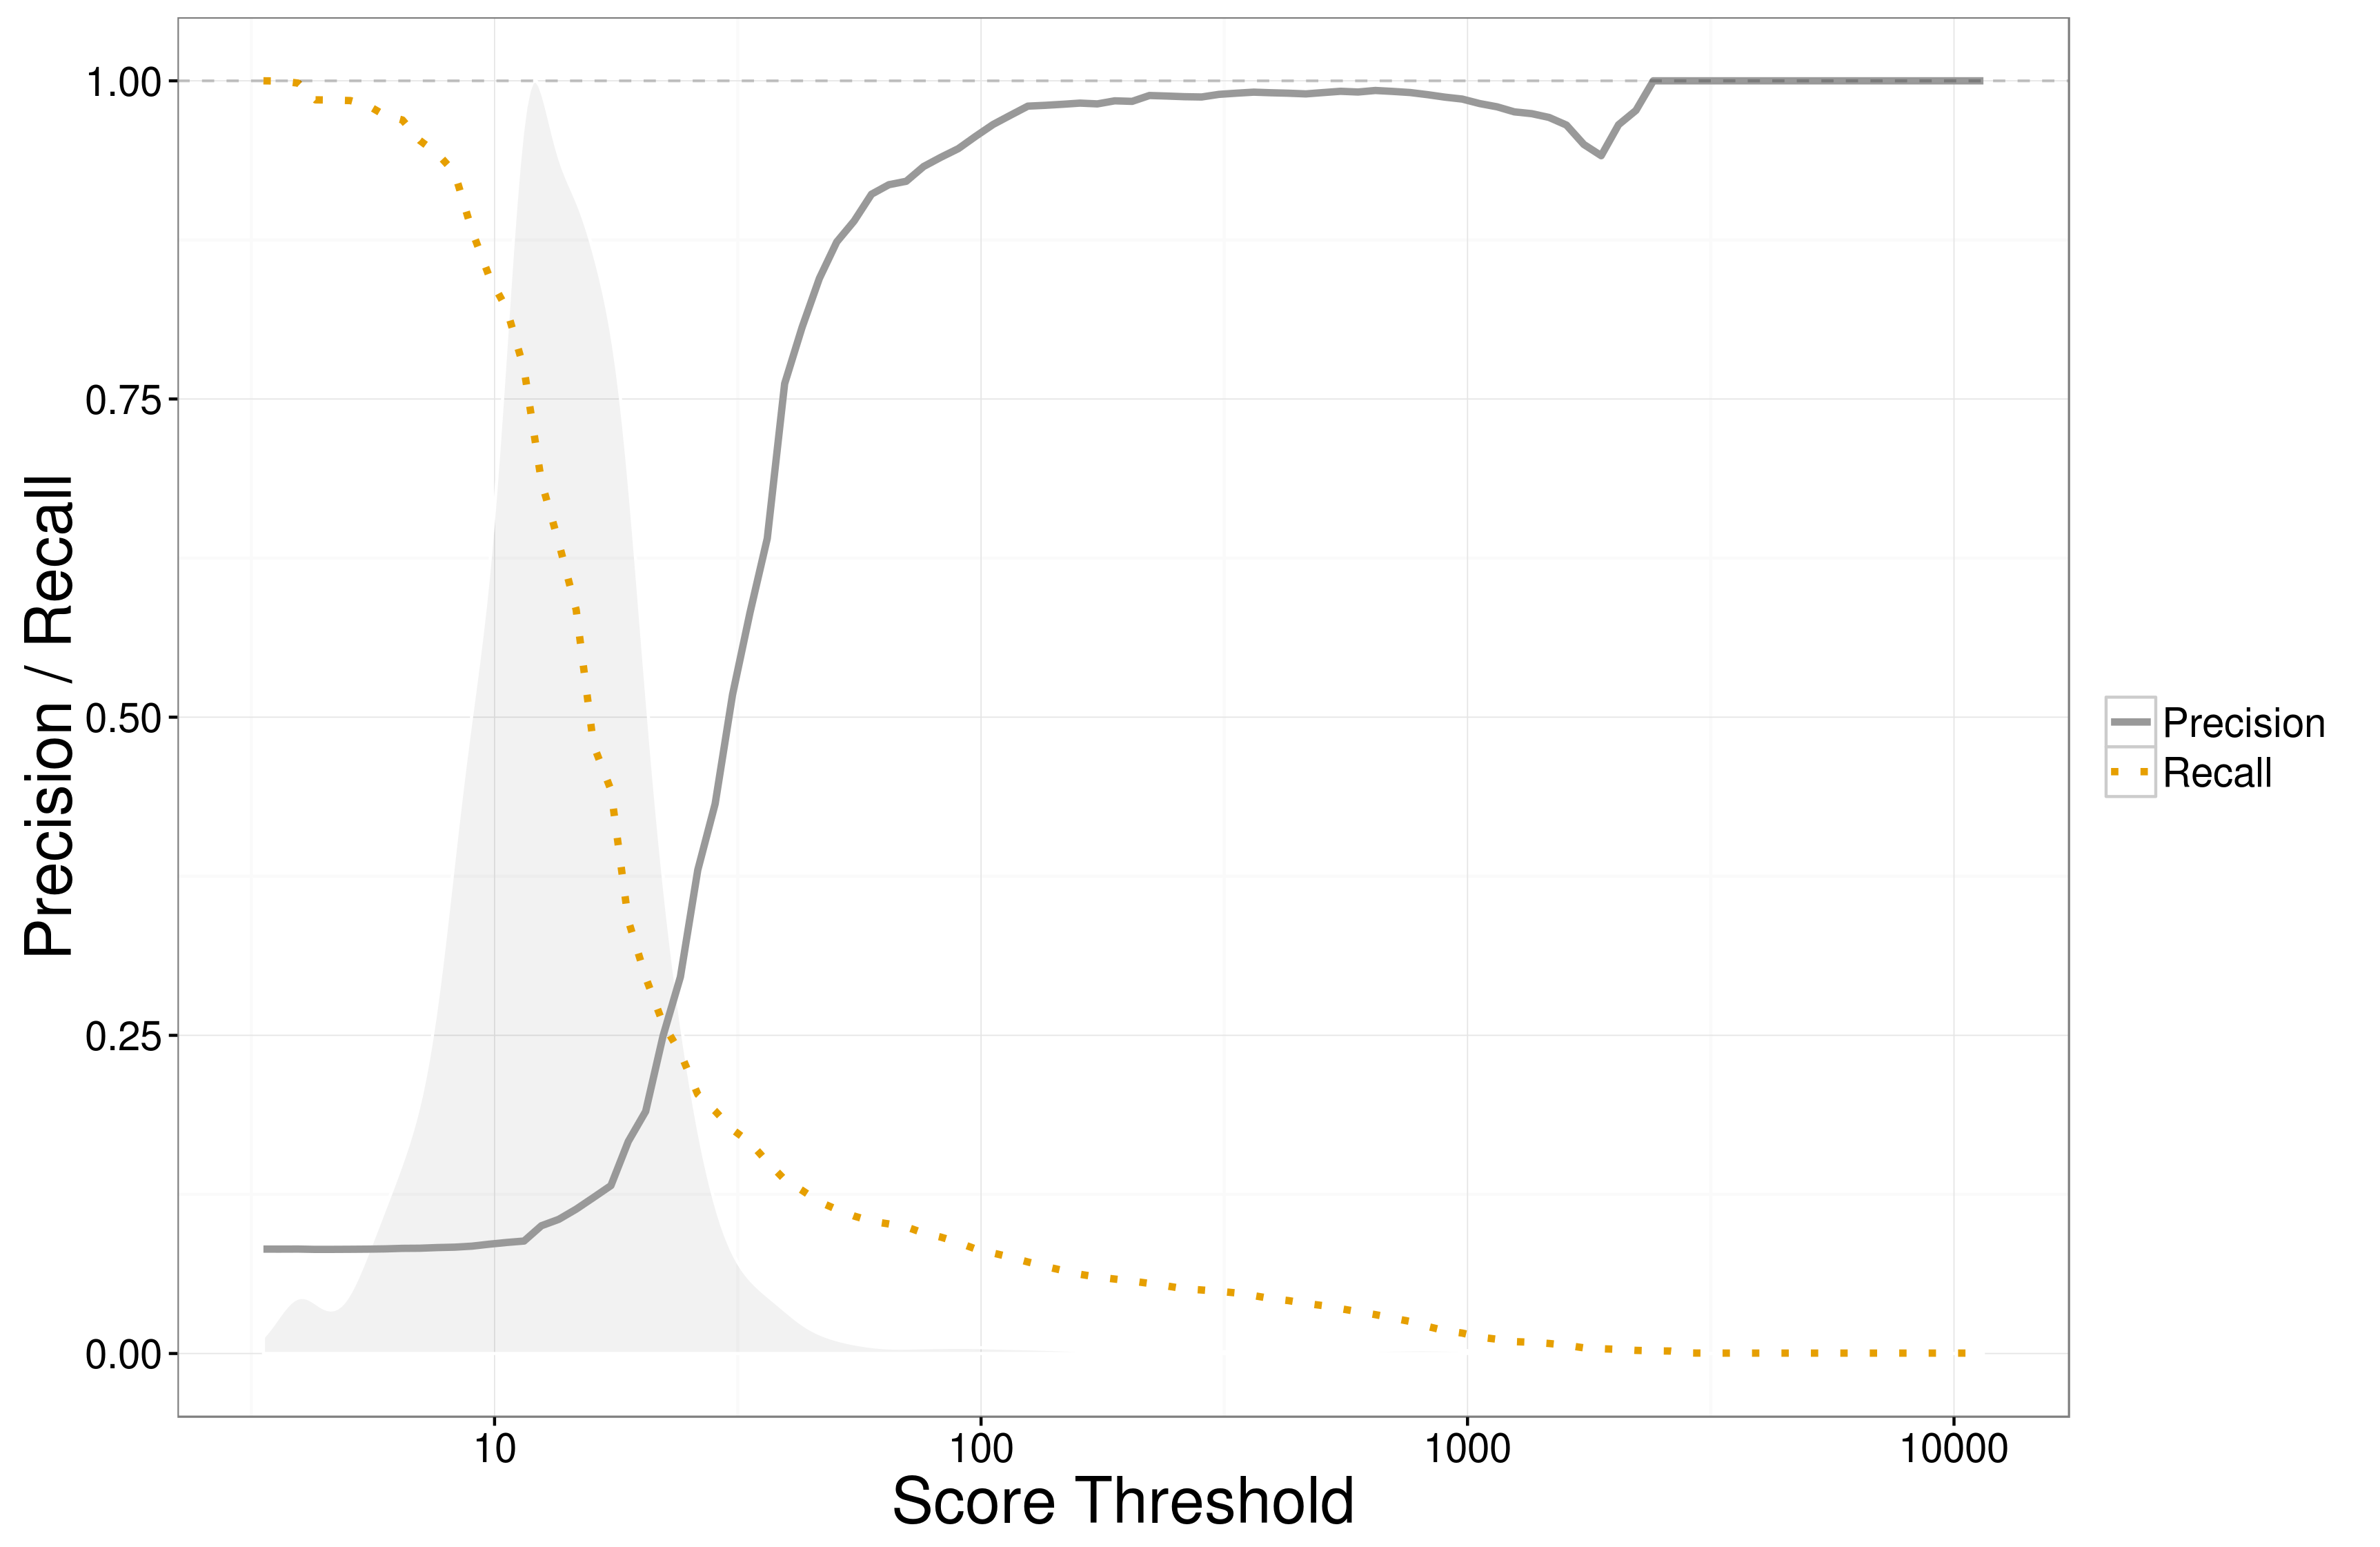
\includegraphics[width=0.8\textwidth]{figures/ncsl_pr_nosplit.png}
\caption{Precision-Recall curve for classifying two bills being in the same
    ncsl table by thresholding the bill-dyad alignment score. The x axis
displays the threshold, the y axis represents precision and recall. The shaded
area in the background displays the frequency distribution of the alignment
scores.}
\label{fig:ncsl_prec_rec}
\end{figure}


\subsection{Diffusion networks and Text re-use}

To evaluate whether text re-use corresponds to the transfer of policy, we test whether the presence of a diffusion network tie between two states is a predictor of text reuse. We use the policy diffusion networks inferred in \citet{desmarais2015}. The diffusion networks were inferred using policy adoption sequences, and the network inference algorithm developed by \citet{gomez2010inferring}. A tie from state $i$ to state $j$ in the diffusion network indicates that state $j$ has frequently emulated state $i$'s policies in the preceding thirty-five years. To calculate an aggregate alignment score for each state-pair we calculate the sum of the natural logs of the alignment scores associated with each pair of bills across the two states. We use the log since a handful of large alignment scores lead to extreme outliers on the original scales. The ``Diffusion Ties'' variable indicates the presence of a diffusion edge between states in the 2008 diffusion network, as measured by \citet{desmarais2015}. The diffusion network in 2008 is inferred using policy adoptions in the 35 years preceding (and excluding) 2008.  There is one observation in the analysis for each of the 1,225 unique state-pairs. Since this is dyadic data, we use a matrix permutation method, quadratic assignment procedure, to calculate $p$-values \citep{krackhardt1988}. As a robustness check, we run the model with both the identity and log link.\footnote{The $p$-values were calculated using 5,000 random matrix permutations.}

% latex table generated in R 3.2.3 by xtable 1.8-2 package
% Wed Sep 21 20:12:14 2016
\begin{table}[ht]
\centering
\begin{tabular}{rrrrr}
\hline
& \multicolumn{2}{c}{Identity Link} & \multicolumn{2}{c}{Log Link} \\
  \hline
 & Coefficient & p-value & Coefficient & p-value \\ 
  \hline
Intercept & -33577305.97 & 0.00 & 10.04 & 0.00 \\ 
  Diffusion Tie & 2423709.31 & 0.05 & 0.27 & 0.10 \\ 
  Coverage & 10938819.90 & 0.00 & 1.38 & 0.00 \\ 
  \hline
\end{tabular}
\caption{Predicting number of alignments in legislation across states with diffusion ties. Coefficients calculated with OLS regression. $p$-values based on 5,000 QAP permuations.}
\label{tab:qap.diffusion}
\end{table}

Results of the dyadic regression are presented in Table \ref{tab:qap.diffusion}. In both specifications there is a positive relationship between the number of diffusion ties and the number of alignments. The relationship is statistically significant at the 0.05 level with the identity link and at the 0.10 level with the log link. Furthermore, the magnitudes of the relationships are substantively significant. With the identity link, the presence of a diffusion tie leads to a 0.25 standard deviation increase in the expected aggregate alignment score.Based on the log link, the addition of a diffusion tie corresponds to a 30\% increase in the expected aggregated alignment score.\footnote{Calculated as $100\times \left[ \exp(0.2683)-1\right] = 30.77$}. These results offer further evidence of the validity of quantifying text re-use as a measure of policy similarity, as the aggregate volume of text re-use between states is positively associated with previously-identified diffusion ties between states.


\subsection{Ideological Distance of Aligned Bills}

In the previous two validity tests, we focused mainly on the policy domain
aspect of policy similarity, rather than ideological similarity. In the third
and final validity test we ask whether we observe a greater volume of text reuse
between bills introduced by legislators who are ideologically similar. For
calculating ideological distance, we rely on latent ideology scores measured by
\citep{shor2011}. The data set contains scores for 20,738 legislators from 50
state legislatures. The \texttt{openstates} API, which we can match to our bills
data, contains data and identifiers on $12,000$ legislators. Of these, we where
able to uniquely match about $8,000$ legislators to their records in the ideal
point data. This allowed us to obtain ideal points for the sponsors of $58\%$ of
bills and $48*10^6$ ($38\%$) pairs of bills. In order to assess the validity of text reuse as a measure of substantive policy overlap, we expect the quality of the alignments to be inversely correlated to the distance between the bills sponsors' ideal points. The ideal points are located on a common scale across all states, the distance between sponsors from different states is therefore meaningful. 

In the following sections we present several analyses to assess this correlation. The ideal point of the bill is derived from the ideal point of the primary bill sponsor. For bills with several primary sponsors we use the average of those sponsors' ideal points to obtain a single measure. Figure \ref{fig:ideology_plot} displays the distribution of ideological distance and log-alignment score for the roughly 50 million dyads in the dataset. Each dot is a hexagonal tile, the color of the tile represents the number of dyads in that area. Two major observations can be made in this plot. First, the vast majority of alignment scores are close to zero. Second, the triangular shape of the distribution indicates the high precision - low recall character of the alignment score discussed above: few bills exhibit meaningful policy overlap with other bills, but in the region of lower ideological distance we observe a greater occurrence of positive outliers, which arise from significant policy overlap. 

In order to investigate this pattern more closely, we additionally calculate
quantile regressions for the relationship between the alignment score and the
ideological distance. Figure \ref{fig:quantile_regression} displays the
coefficients from quantile regressions on a sequence of quantiles from the
median to the 0.995th quantile. Confidence intervals are calculated by resampling bills, which represents an implementation of the clustered nonparametric bootstrap \citet[see e.g.][]{harden2011bootstrap}. Coefficients significant at the 95\% level are displayed in black, insignificant coefficients are grey. We see that there is only a very weak relationship between the ideological similarity of bill sponsors and the median alignment scores between bills. However, as the quantile we model increases we see that the relationship grows strong and negative in magnitude, and is statistically significant. These results both validate the use of text reuse as a measure of policy similarity, and reinforce the high precision and low recall nature of text reuse as a measure of policy similarity.


\begin{figure}[ht!]i
    \centering
    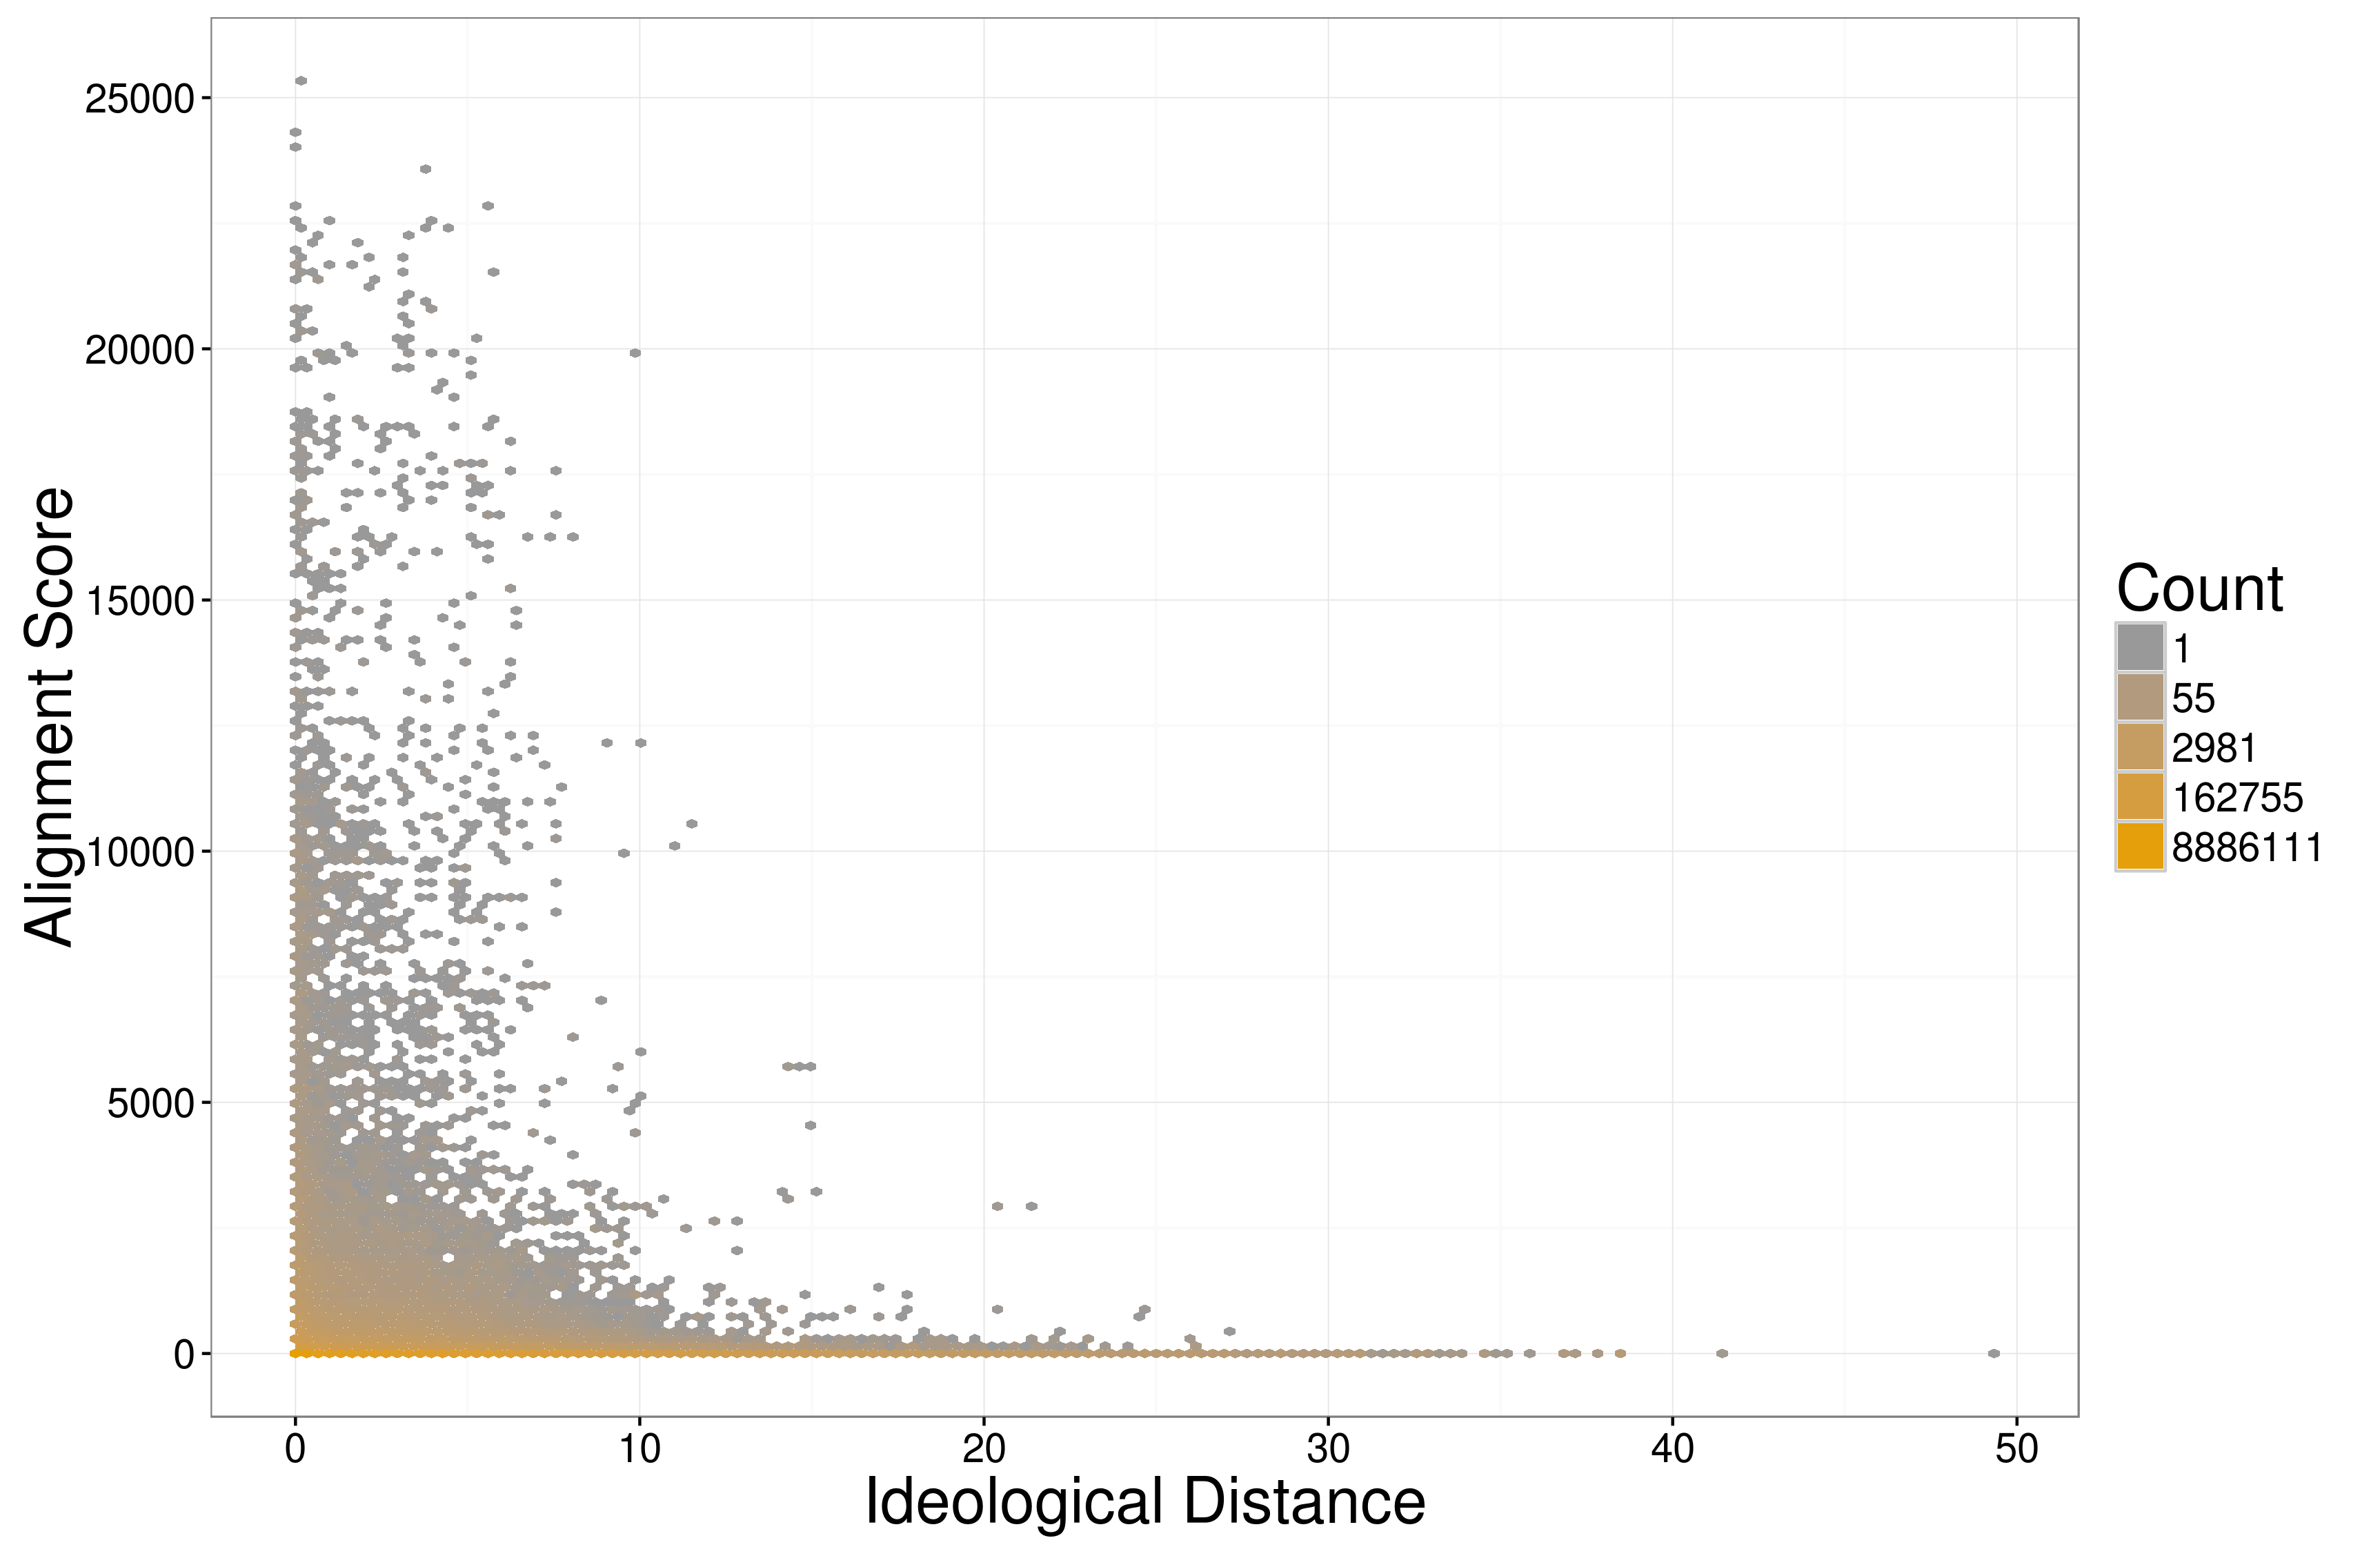
\includegraphics[width=0.8\textwidth]{figures/ideology_plot.png}
    \caption{Hexbin plot of alignment score and ideological distance of all 50 million bill dyads.}
    \label{fig:ideology_plot}
\end{figure}

\begin{figure}[ht!]
    \centering
    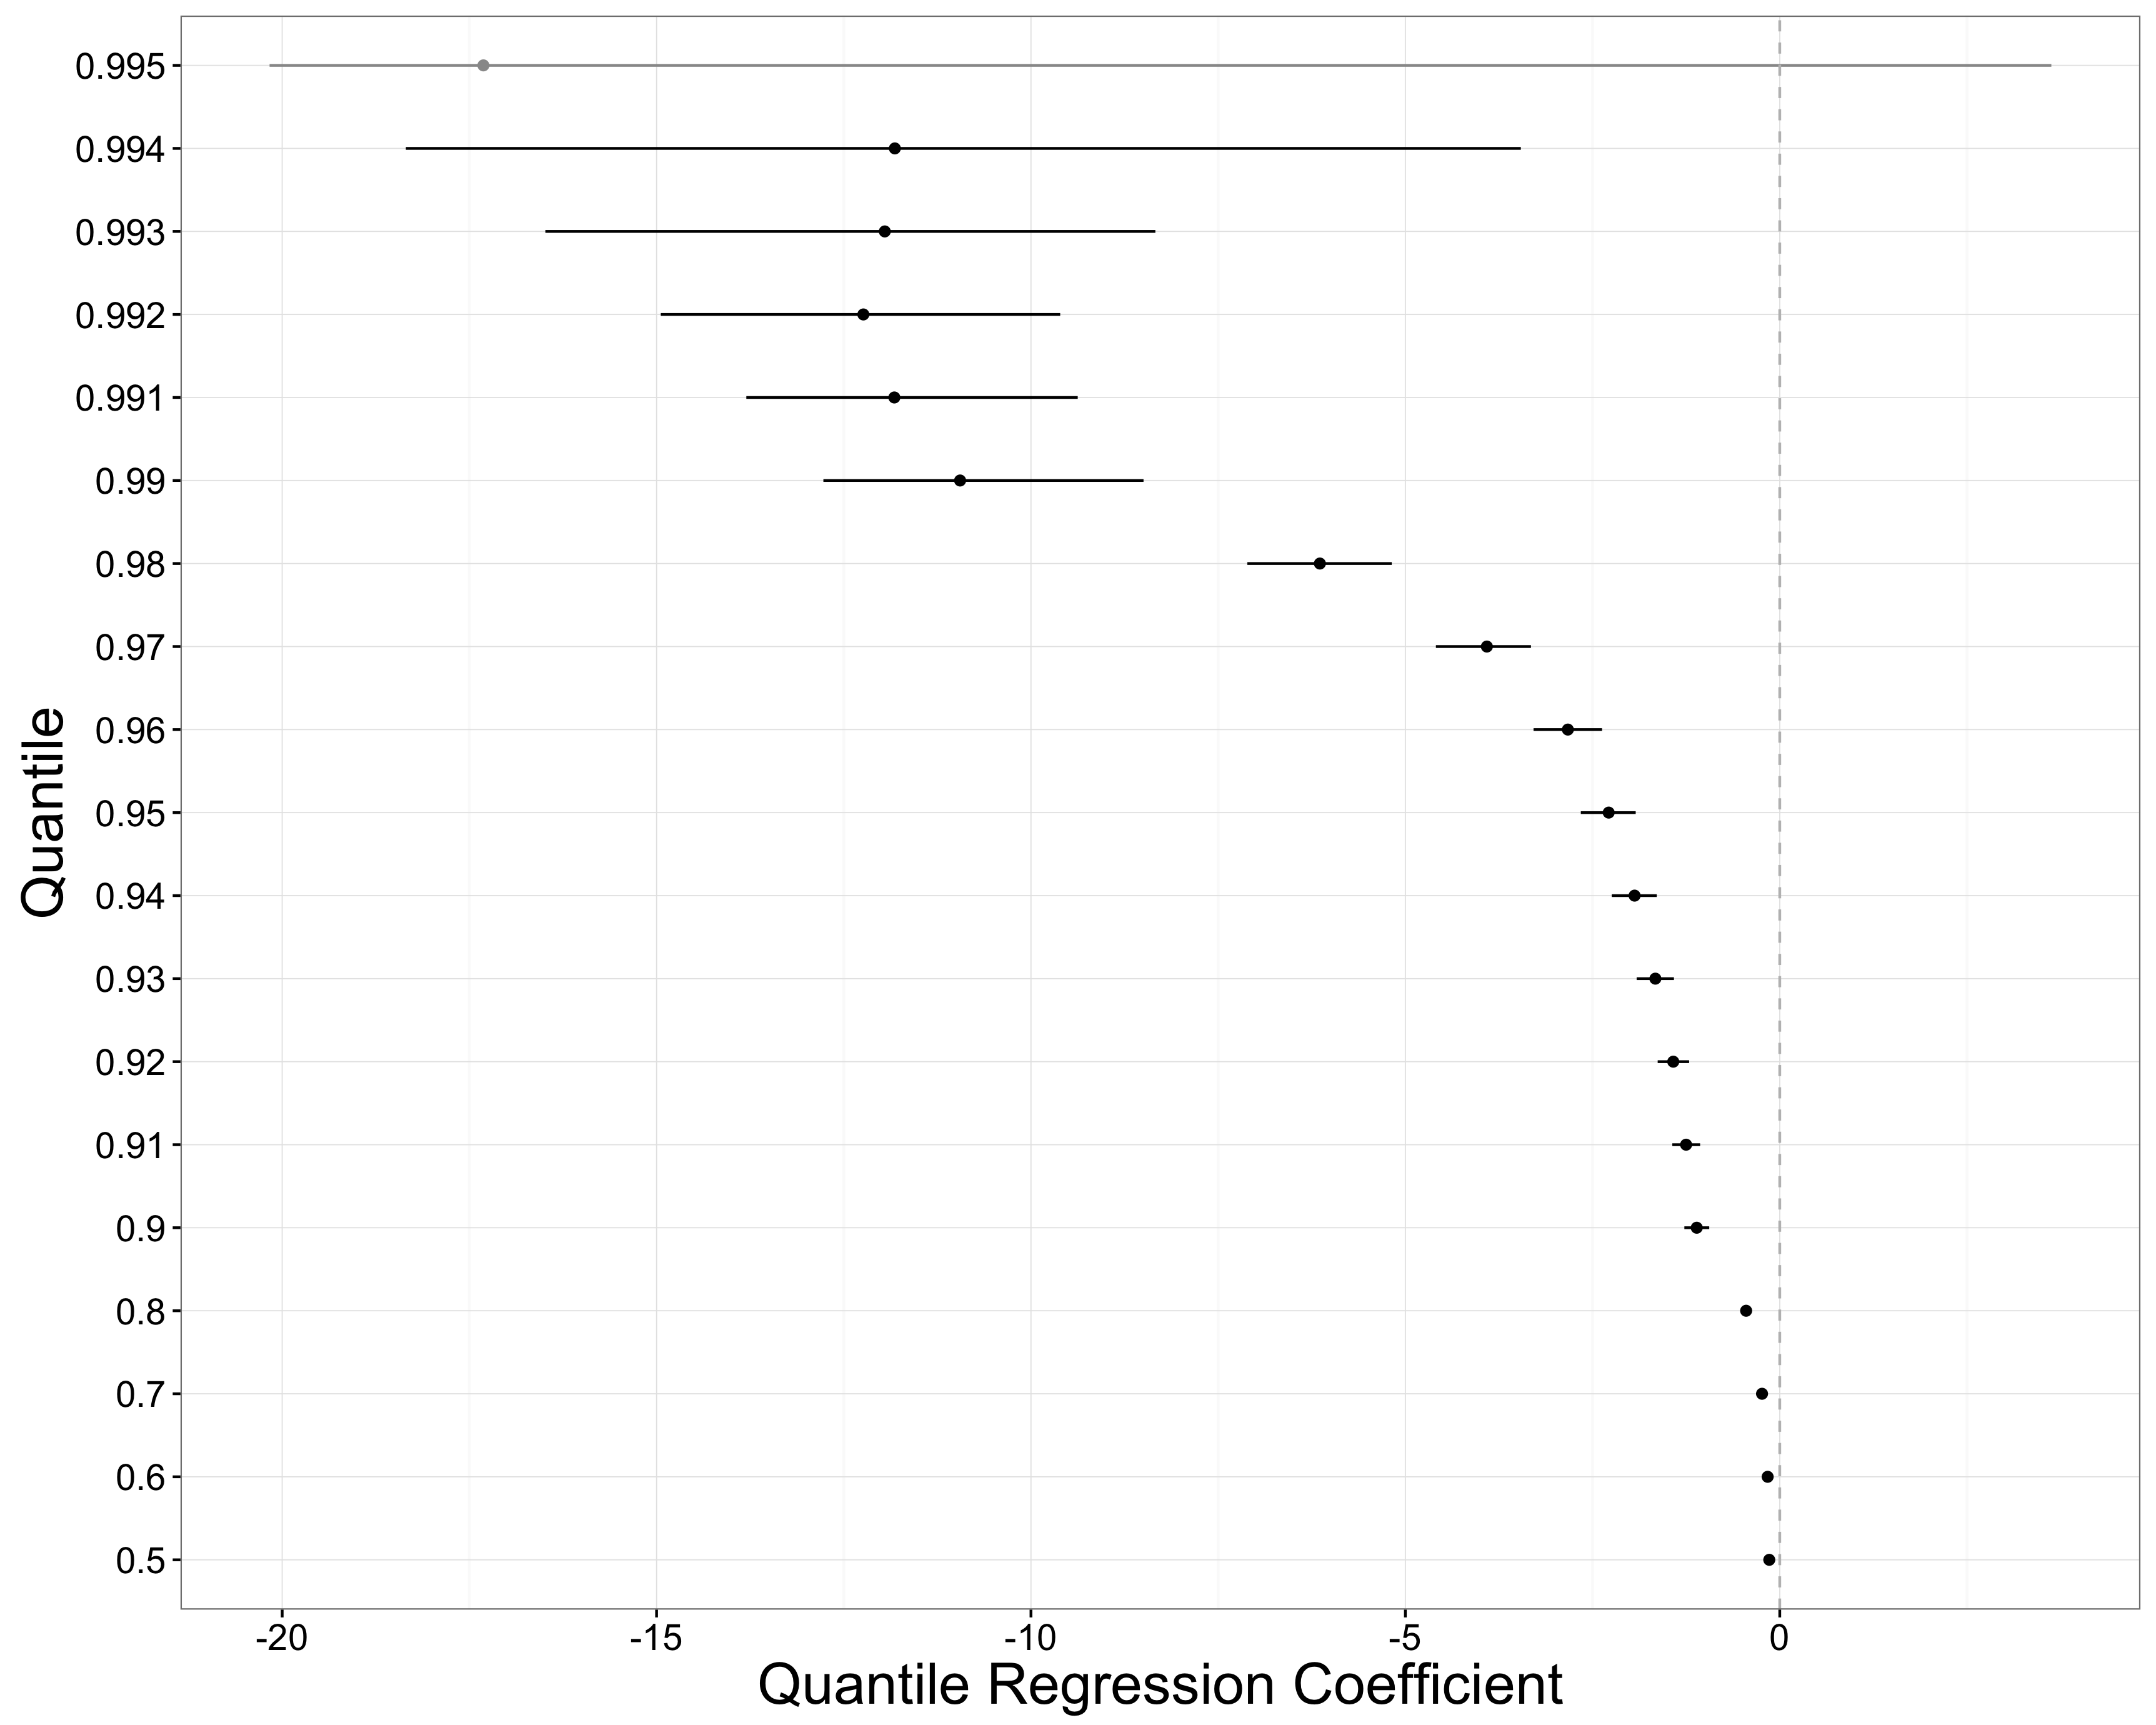
\includegraphics[width=0.8\textwidth]{figures/quantile_regression.png}
    \caption{Coefficients of quantile regression for alignment score on
    ideological distance. Dots indicate the point estimate. Horizontal bar
represent 95\% confidence intervals obtained via the clustered bootstrap, [using
1200 iterations]. Note that the x-axis is not in a natural scale}
    \label{fig:quantile_regression}
\end{figure}


\clearpage


\section{Conclusion}
Scholarship on public policy and legislative politics relies heavily on measuring the content of legislation, especially with a relative or comparative approach. Manual comparison of bills is prohibitively time consuming when it comes to covering a large proportion of legislation introduced in one or more legislatures. We show that the automated detection of similar text strings in bills provides an effective approach to comparing bill contents. The log alignment scores serve as a highly valid summary measure of the similarity of two bills. We show high validity of this measure in three complimentary tests. First, it correlates with the presence of a diffusion tie inferred from patterns of policy diffusion. Second, it correlates with the ideological similarity between bill sponsors. Third, it exhibits extremely high precision in predicting whether two bills are listed in the NCSL policy area tables. We demonstrate the potential for using this data to test new or unexplored hypotheses on lawmaking in the states by testing whether bill text similarity correlates with campaign contributions to US state legislators.

The log alignment scores we derive provide a resource for scholars to test hypotheses of the causes and consequences of the introduction and adoption of similar policies---a measure which crosses different policy areas, states, and time. Where and when do similar policies cross state borders? Which legislators introduce similar legislation? Does lobbying by pressure groups result in the adoption of similar policies across states? Do similar patterns of campaign contributions to legislators predict similar policies in proposed legislation? Questions such as these can be directly investigated using the policy similarity measures we introduce. 

A consistent result in our analysis is that the measure of policy similarity based on text reuse is high precision and low recall.  As such, in future research we advise scholars to focus on upper quantiles of the distribution of alignments, especially when considering measurements at the bill-level. This can be done through the use of quantile regression, or through thresholding on high alignment scores (e.g., 50+) to indicate the presence of highly similar policy proposals in legislation.

%\clearpage

\bibliographystyle{chicago}
\bibliography{bibliography}

\clearpage

\section*{Appendix}

\textit{Sketch for a proof that SW alignment is globally optimal}

Notation $F_i$ is the alignment of size $i$ with $i = 1,2,...,(n + k - 1)$. $S(F_i)$ is the score of the alignment.

First show that the score in each cell is optimal:
\begin{enumerate}
\item There are three options for $F_1$ (Gap in $\mathcal{A}$, Gap in $\mathcal{B}$, . This alignment is optimal when $S(F_1)$ is maximized
\item Every alignment's score $S(F_i)$ with $i > 1$ when maximized, is composed of the score of the `one-shorter' alignment $S(F_{i-1})$ and the score of the $i$-th element. If not the score could be increased by choosing a different $F_{i-1}$ that has a higher score.
\item The dp matrix contains all possible alignments. Since every cell is optimal, the highest score in the dp matrix must be globally optimal
\end{enumerate}


\end{document}




